\documentclass[12pt]{article}
\usepackage{graphicx}
\usepackage{hyperref}
\usepackage{amsmath}
\usepackage{amssymb}
\usepackage{siunitx}
\usepackage[numbers, square, sort&compress]{natbib}


\begin{document}
\title{Chapter 14: Special Topics in Molecular Docking}
\author{Elvis Martis}
\date{}
\maketitle

\section{Introduction}

Classical small–molecule docking assumes a single, rigid, or modestly flexible, protein target and a single non-covalent ligand that occupies a well–defined binding pocket.  In practice, however, many of the most interesting and pharmacologically relevant systems violate one or more of these assumptions: ligands can form covalent bonds with their targets, two or more proteins and a bifunctional molecule can assemble into a ternary complex, or several ligands share a binding site and interact cooperatively or competitively.  Most of these topics are outside the scope of routine molecular docking. Nevertheless, as these are increasingly gaining attention, we dedicate a separate chapter to discuss them. For the sake of this chapter, we label the systems and case studies as  \emph{difficult} systems and show how molecular docking has been extended, both conceptually and algorithmically, to handle them.

In this chapter, we focus on three major classes: covalent docking, docking for PROTAC (proteolysis‐targeting chimera) design, and simultaneous docking of multiple ligands into a single protein binding site.  Each section introduces key theoretical foundations, docking protocols, and pitfalls. We have curated a set of case studies to showcase how these difficult systems are handled and what the docking workflow looks like. Along the way, we highlight methodological innovations in reactive scoring functions, constrained protein–protein docking, and multi–ligand search algorithms, that collectively extend the utility of docking far beyond the traditional one–protein/one–ligand systems

\section{Covalent Docking}

In covalent inhibition, the ligand forms a chemical bond with a specific nucleophilic residue, typically a cysteine, serine, lysine, or catalytic threonine. The binding process is therefore at least a two–step process: an initial non-covalent recognition step, followed by a chemical reaction leading to a covalent adduct.  Classical docking treats the potential energy surface as a function of non-bonded terms, such as electrostatics, van der Waals, and solvation, and thus cannot directly represent bond formation or changes in connectivity.

 Covalent docking\cite{CH14_CovalentDockingReview2015,CH14_CovalentToolSelection2019} strategies encode the reaction in one of three broad ways.  
 \paragraph{Attachment or link–atom:} Here, the covalent bond is predefined between the ligand warhead and the target residue, and docking explores only the post–reaction complex using modified topologies and tailored scoring terms. 
 
 \paragraph{Two-step or reactive:} In this approach, the program samples pre–reaction binding modes that geometrically satisfy distance and angle criteria for nucleophilic attack, then converts those poses that pass into covalent complexes that are rescored with a covalent energy term.  
 
 \paragraph{Hybrid quantum–mechanical/molecular–mechanical:} This QM/MM method explicitly optimises the reaction coordinate in the binding site, albeit at much higher computational cost.


\subsection{Algorithms and tools}

Several covalent docking methods show different trade–offs between speed and accuracy.  Early covalent virtual screening protocols embedded a covalent linker into the ligand topology and primarily used classical force fields with modified bonding terms to model the covalent adduct. Later methods introduced explicit reactive sampling, in which the search first identifies orientations that satisfy geometric constraints for a predefined reaction type, for example, Michael addition to an acrylamide warhead, then builds the covalent complex and refines it\cite{CH14_CovalentLargeLibraries2014}. WIDOCK\cite{CH14_WIDOCK2021}, for instance, defines a library of reaction templates, uses a reactive docking engine to generate pre–reaction complexes, and then evaluates candidate poses using an empirical scoring function supplemented by penalty terms for poor reaction geometry. In benchmarks on cysteine-targeted electrophiles, this reactive approach retrieved known covalent inhibitors with higher enrichment than a purely non-covalent variant of AutoDock, particularly when diverse warheads were present in the screening library.  Similarly, HCovDock\cite{CH14_HCovDock2023} combines incremental ligand construction with a covalent bond-aware scoring function and achieved redocking success rates above 70\% across more than two hundred diverse complexes, outperforming several widely used commercial covalent docking tools.

An orthogonal direction is to improve the description of the chemical step using quantum-mechanical (QM) or semiempirical methods. Hybrid schemes such as CovCIFDock\cite{CH14_CovCIFDock2025} dock the pre–reaction complex with a flexible classical docking engine and then perform QM/MM minimisation to form and refine the covalent bond. On large benchmarks containing covalent inhibitors of proteases, kinases, and nuclear export receptors, such workflows could reproduce crystallographic poses within $\sim$2 \r{A}, while retaining accuracy comparable to that of leading commercial programs. More general hybrid quantum/classical docking workflows based on Attracting Cavities\cite{CH14_HybridQMClassDocking2025,CH14_rohrig2023attracting,CH14_chaskar2017fly} have demonstrated that inclusion of semiempirical or density functional theory (DFT) for the reactive centre improves pose prediction on diverse covalent test sets, particularly for challenging systems with ambiguous electron densities.

Covalent docking is no longer restricted to small molecules: there are reports to covalently docking peptides, which add the complexity of high ligand flexibility and folding.  The central ideas, such as explicit warhead parameterisation, reaction templates, and covalent scoring, remain the same; however, they must be coupled to advanced sampling of peptide backbone and side–chain conformations, often using hierarchical or fragment–based approaches\cite{CH14_Covpepdock}.

\subsection{General covalent docking workflow}

 A robust covalent docking workflow typically proceeds through the following steps:

\begin{enumerate}
  \item \emph{Define the reactive residue and mechanism}: Identify the nucleophilic residue, for example, Cys145 in SARS–CoV–2 3CL protease\cite{CH14_Gu3CL}, and specify the reaction type, such as Michael addition, nucleophilic substitution, or reversible boronate formation.  
  \item \emph{Prepare the protein}: Build the side–chain in the appropriate protonation/tautomeric state and remove non-essential crystallographic waters unless they are known to participate directly in the reaction or binding.  
  \item \emph{Annotate warheads}: Label electrophilic atoms, specify their connectivity to the protein in the post–reaction state, and assign parameters, like partial charges and bond orders, required by the docking engine.  
  \item \emph{Choose sampling mode}: For small warhead libraries, reactive, two–step, protocols are often preferred because they enforce better reaction geometry. For very large libraries, post–reaction docking with constrained bond vectors is more efficient.  
  \item \emph{Score and filter}: Use a scoring function that combines non-covalent terms with penalties for strained reaction geometries or physiologically irrelevant protonation states. In many workflows, hits are further filtered by physicochemical rules or warhead reactivity heuristics.  
  \item \emph{Post–processing}: Selected poses are refined with local minimisation and, where feasible, short molecular dynamics (MD) simulations to ensure the covalent adduct is sterically and dynamically stable.
\end{enumerate}

It must be kept in mind that the \emph{best} non-covalent pose may not necessarily translate to the \emph{best} covalent pose.  For example, the pre–reaction complex that maximises hydrophobic contacts may place the warhead in a geometry that makes nucleophilic attack difficult or nearly impossible. Whereas a slightly less favourable non-covalent pose with good attack angle and distance is more likely to translate into favourable covalent bond formation. Covalent docking, therefore, forces one to think simultaneously about supramolecular recognition and chemical reactivity.

\subsection{Case study: Covalent fragments against a serine hydrolase}

A classic example is the use of covalent docking to discover electrophilic fragments targeting enzymes such as serine hydrolases or $\beta$–lactamases. A library of several thousand electrophilic fragments was docked covalently into the active sites of AmpC $\beta$–lactamase\cite{CH14_babaoglu2008comprehensive}, and various kinases using a dedicated covalent virtual screening protocol. The hits were subsequently validated crystallographically as valid chemical probes. As these fragments were small and weak in their non-covalent interactions, classical docking alone would have failed to identify them as potential binders. However, inclusion of the covalent bond and appropriate geometric constraints enabled the virtual screen to recover low–affinity electrophiles that nonetheless formed stable covalent complexes.

A simplified version of the protocol is shown as follows:

\begin{enumerate}
  \item \emph{Choice of the system}: Select a serine hydrolase with a high–resolution structure containing a covalent inhibitor, for example, a $\beta$–lactam or fluorophosphonate, to serve as a template for covalent geometry.  
  \item \emph{Template extraction}: Remove the covalent ligand and record the bond vector and angles between the active–site serine oxygen and the scissile carbon atom.  
  \item \emph{Fragment library}: Curate a small library, perhaps hundreds to thousands, of electrophilic fragments, for example, acrylamides, chloroacetamides, and sulfonyl fluorides, with diverse scaffolds with shared warheads.  
  \item \emph{Covalent docking}: Use a covalent docking program, or a non-covalent program equipped with a covalent plug–in, to generate covalent adducts between each fragment and the catalytic serine, enforcing approximate template–based reaction geometry.  
  \item \emph{Scoring and triage}: Rank-order poses by covalent score. Visually inspect the top few poses for reasonable complementarity to the oxyanion hole, absence of severe steric clashes, and plausible interactions with conserved active–site residues.  
  \item \emph{Experimental validation}: Select a subset of fragments for synthesis or purchase. Assess covalent labelling using mass spectrometry or activity–based profiling.
\end{enumerate}


\section{Docking for PROTAC Design}

PROTACs are heterobifunctional (\textbf{Figure \ref{fig:protac}B}) molecules that recruit an E3 ligase to a target protein, triggering ubiquitination and proteasomal degradation(\textbf{Figure \ref{fig:protac}A}).  Structurally, a PROTAC contains a scaffold that binds the target, a ligand for an E3 ligase, such as VHL or cereblon, and a linker that connects the two moieties.  
The pharmacologically relevant species is a ternary complex comprising the target protein, the E3 ligase, and the PROTAC; the stability and geometry of this assembly strongly influence degradation efficiency.

\begin{figure}[hbt!]
    \centering

    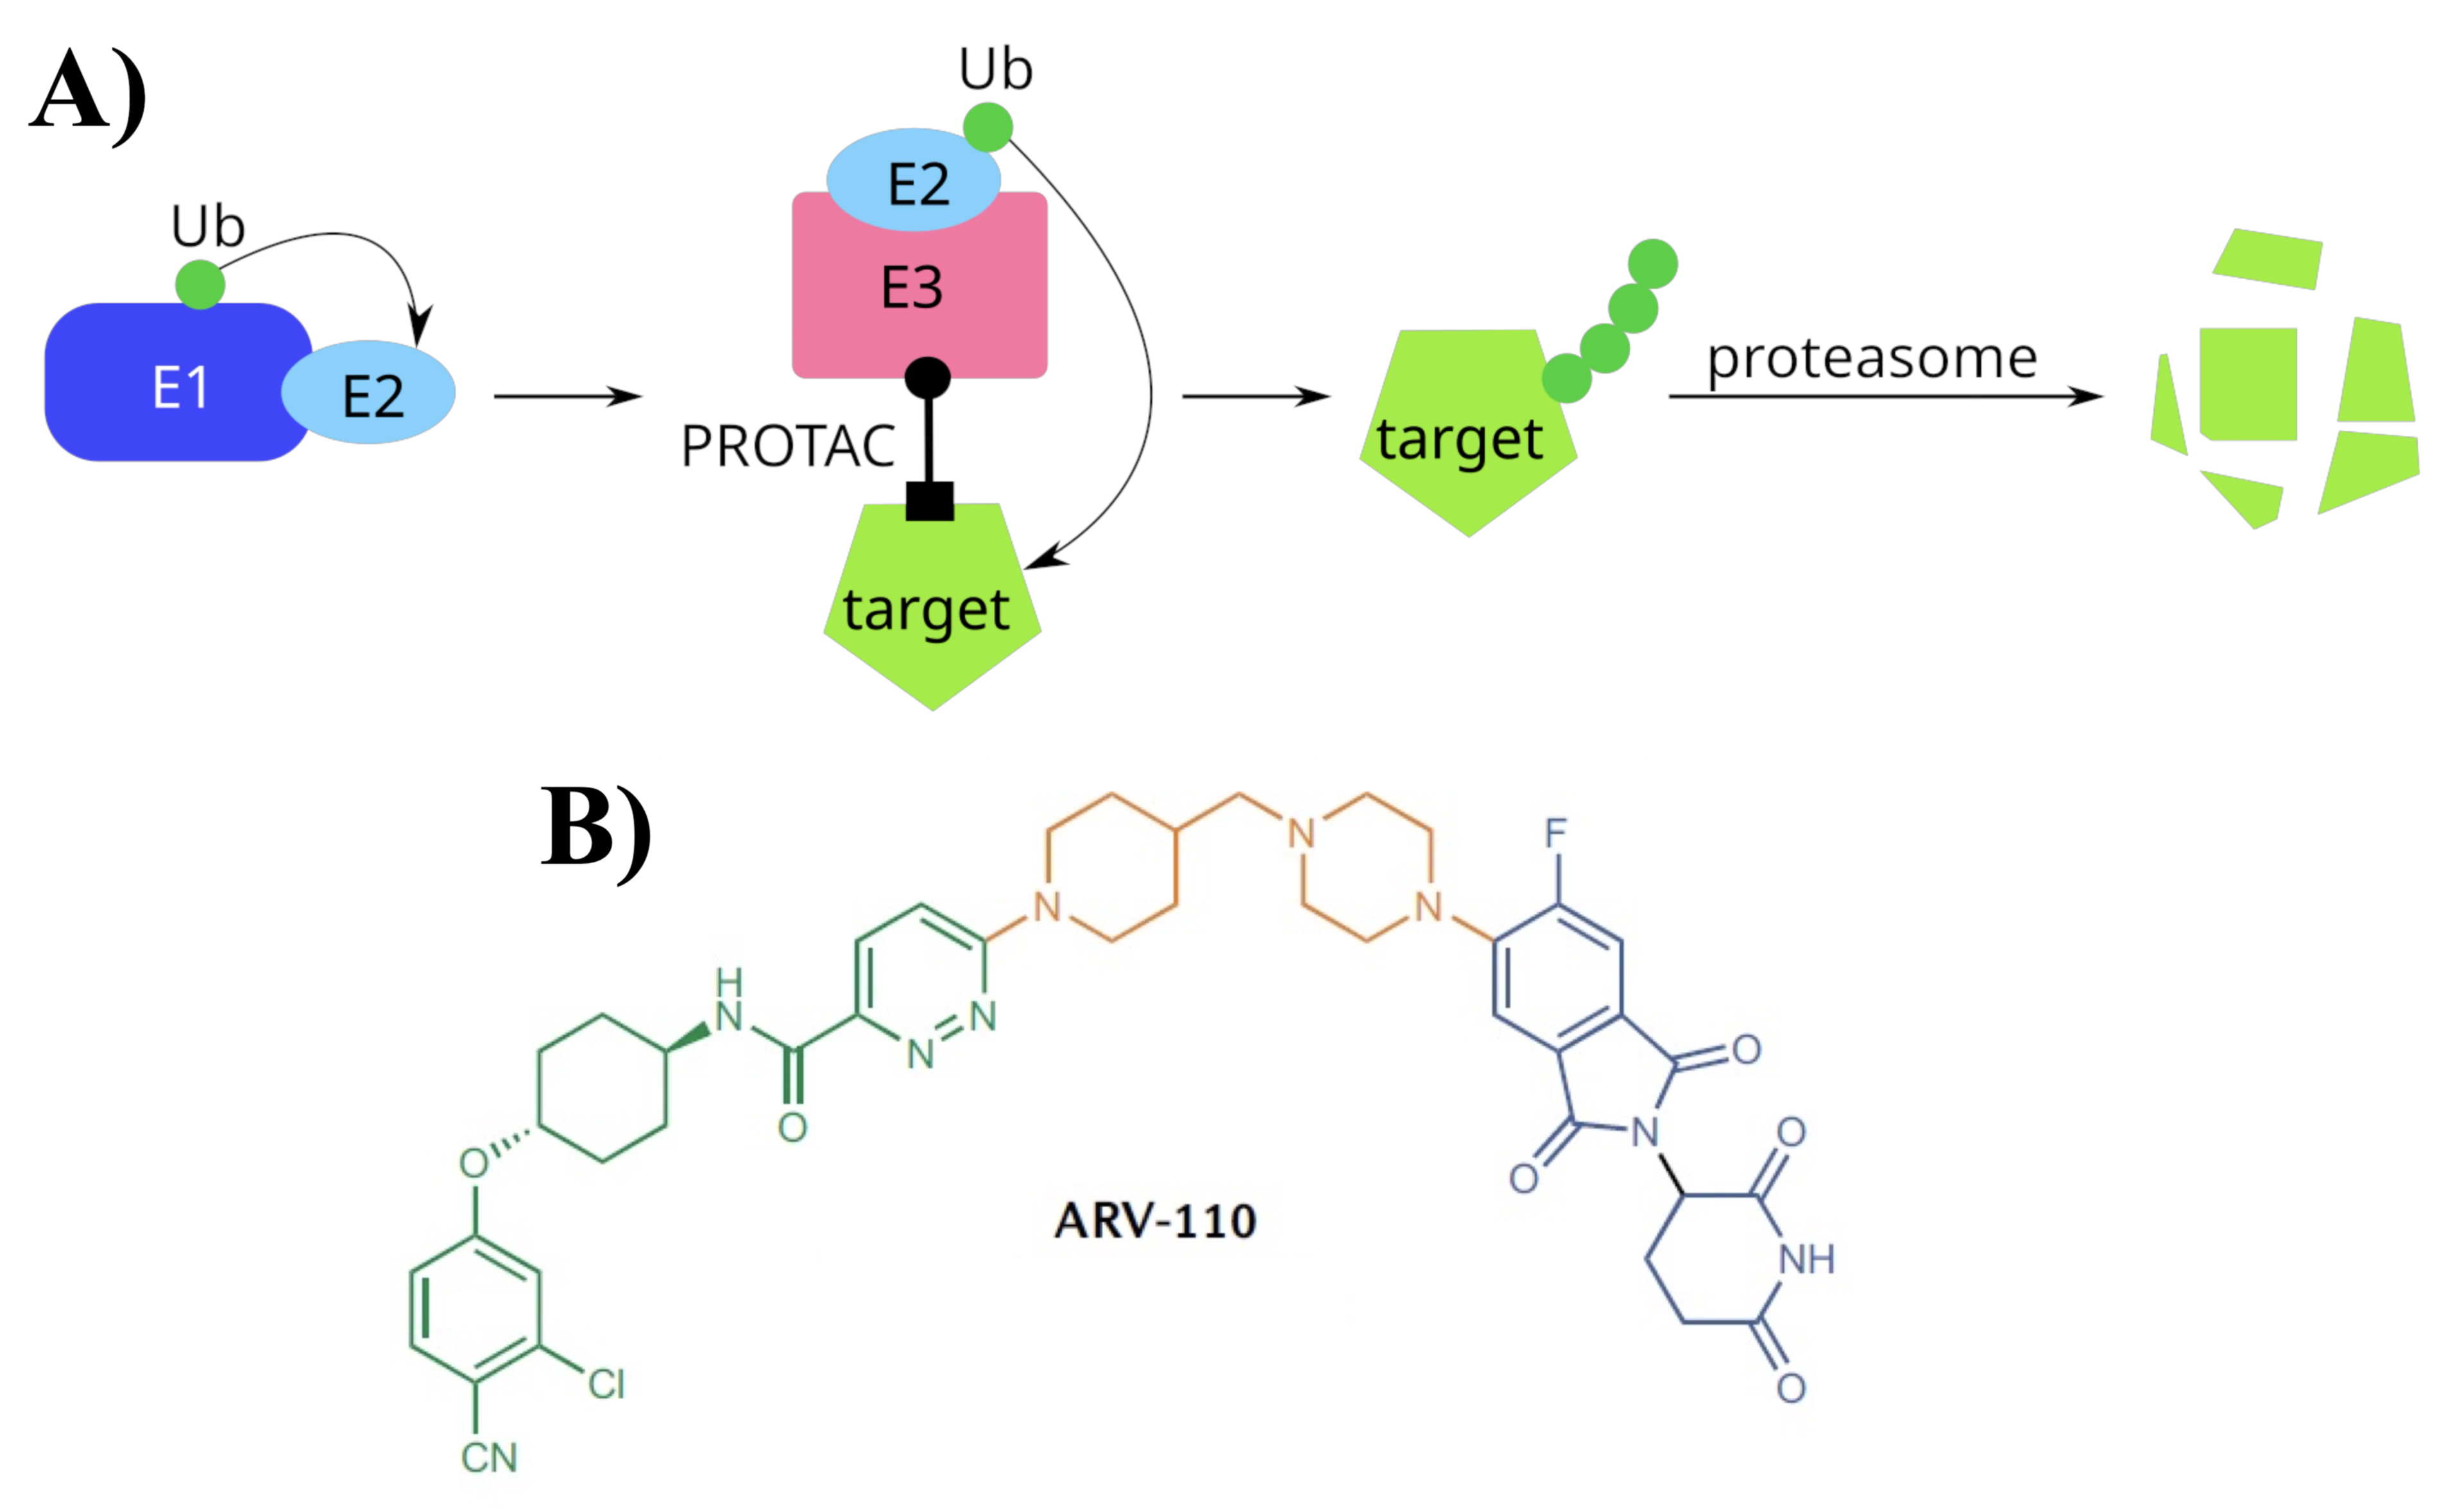
\includegraphics[width=1\textwidth]{PROTAC.jpg}

    \caption{\textbf{A.} Proteolysis targeting chimera mechanism. E1, E2, E3: ubiquitination enzymes; Ub = ubiquitin; PROTAC = proteolysis targeting chimera; target = protein to be degraded \textbf{B.} Chemical structure of ARV-110, an investigational, orally bioavailable PROTAC. Ligands targeting androgen receptors (green), linkers (orange), and ligands targeting E3 CRBN (blue). This image is partially reproduced under the Creative Commons CC0 1.0 Universal Public Domain Dedication} 
\label{fig:protac}
\end{figure}

Docking for PROTACs is intrinsically more complex than conventional docking for several reasons.  First, one must consider protein–protein interactions between the target and ligase, which may be weak or absent in the absence of the PROTAC. Second, the PROTAC must adopt a conformation that simultaneously satisfies the binding requirements of both pockets and accommodates the protein–protein interface. Third, the space of linker conformations and protein orientations is very high–dimensional, so classical sampling is computationally prohibitive. These issues mean that simple sequential docking of the two monovalent ligands into their respective binding sites, with a generic linker built afterwards, often fails to reproduce crystallographic ternary complexes or to correlate with observed degradation efficiencies\cite{CH14_Drummond2020,CH14_PRosettaC2020}. 

To address these challenges, a number of structure–based modelling strategies have been developed that combine constrained protein–protein docking, PROTAC-aware small-molecule docking, and MD simulation\cite{CH14_flt3protac2025,CH14_megaprotac2025}. These approaches differ in technical details but share a common philosophy: first generate ensembles of plausible protein–protein complexes that can, in principle, be bridged by the PROTAC. Then explicitly model the PROTAC within those arrangements and rank resulting ternary complexes using a combination of interface and small–molecule scores.

\subsection{Representative computational Workflow}

One of the approaches, adopted by PRosettaC\cite{CH14_PRosettaC2020}, begins from two binary complexes: target-ligand and E3–ligand. Global protein–protein docking is then performed under distance constraints derived from the linker's known attachment points, generating multiple coarse-grained orientations of the target relative to the E3 ligase.  Next, Rosetta–based local docking\cite{CH14_gray2003protein} refines the protein–protein interface and builds candidate PROTAC conformations that satisfy both binding pockets and linker geometry. These models are clustered and ranked to identify ternary complexes that resemble experimentally solved structures\cite{CH14_Drummond2020}.

In another strategy, the workflow integrated static ternary complex modelling, induced–fit docking, and MD simulations to design VHL–mediated PROTACs targeting the kinase FLT3\cite{CH14_flt3protac2025}. Here, the initial ternary templates were generated by protein–protein docking with MOE and PRosettaC\cite{CH14_PRosettaC2020}, followed by induced–fit docking of PROTACs into each template. Subsequently, MD simulations were employed to check the stability of the ternary complexes and to analyse interface contacts that correlate with degradation potency. Importantly, the results showed that models built in this way could qualitatively reproduce experimental degradation trends across a small series of PROTACs with varying linkers and ligands.

More recently, high–throughput pipelines such as MEGA PROTAC\cite{CH14_megaprotac2025}  have been reported to systematically sample many possible protein–protein complexes, and PROTAC poses using fast FFT–based docking engines.  In MEGA PROTAC, large numbers of protein–protein docking solutions are generated with MEGADOCK, filtered using sequential criteria and rank aggregation, and finally combined with exhaustive PROTAC docking into the selected protein–protein complexes. This type of approach aims to support virtual screening of large PROTAC libraries against structurally characterised target–ligase pairs.

Benchmarks comparing different methods have shown that specialised docking pipelines such as PRosettaC can outperform more generic structure prediction tools\cite{CH14_PRosettaCAf3_2025}, including recent deep learning–based models, when evaluated on their ability to reproduce ternary complex geometries and interface quality metrics.

\subsection{General PROTAC docking workflow}

A PROTAC docking workflow can be described in the following steps:

\begin{enumerate}
  \item \emph{Collect structural data}: Obtain high–resolution structures of the target protein bound to a suitable ligand or close analogue, and of the E3 ligase bound to its recruiter ligand, for example, VHL–ligand complexes.  
  \item \emph{Define attachment points}: Identify the atoms on the target-ligand and ligase-ligand that will be connected by a linker. Measure approximate distances between these positions by superimposing the binary complexes in various orientations.  
  \item \emph{Protein–protein docking under distance constraints}: Use a protein–protein docking to generate plausible orientations of the target relative to the ligase, enforcing soft or hard constraints on the linker attachment points, for example, distances within a tolerance compatible with the planned linker length.  
  \item \emph{Build PROTAC conformations}: For each promising protein–protein orientation, construct PROTAC conformers that bridge the two pockets, either by explicit linker sampling or by a small molecule docking method that can handle long, flexible ligands.  
  \item \emph{Local refinement and scoring}: Refine the ternary complex using local docking or energy minimisation. Score models using a combination of protein–protein interface energy, ligand strain, and poses that satisfy key pharmacophoric contacts in both subpockets.  
  \item \emph{MD–based validation}: For top–ranked ternary complexes, perform short MD simulations to assess the stability of the interface and PROTAC conformations.  
  \item \emph{Relating models to degradation data}: Where experimental degradation assays are available, correlate computed metrics, for example, interface area, number of PROTAC–mediated contacts, or residence time of the ternary complex, with observed degradation efficiencies.
\end{enumerate}


\subsection{Case study: Designing VHL‐mediated PROTACs against FLT3}

This study aims to design VHL–mediated PROTACs targeting the kinase FLT3\cite{CH14_flt3protac2025}, a clinically relevant target in acute myeloid leukaemia. The objective was to model ternary complexes comprising FLT3, VHL, and a series of PROTACs sharing the same ligands but differing in linker composition, and to rationalise why some PROTACs showed superior degradation properties experimentally.

The computational protocol is outlined as follows:

\begin{enumerate}
  \item \emph{Binary templates}: X–ray structures of FLT3 bound to a small molecule inhibitor and VHL bound to its recruiter ligand were used to align structures in several plausible ways to bring linker attachment points into approximate proximity.  
  \item \emph{Static ternary models}:  Using MOE and PRosettaC for protein–protein docking, various FLT3–VHL orientations were systematically explored. The distance between attachment atoms within ranges compatible with the planned linker length was used as a filter to discard orientations warranting linkers beyond this range. 
  \item \emph{Induced–fit docking of PROTACs}: For each static protein–protein orientation, an induced–fit docking of the full PROTAC was performed, allowing side–chain flexibility near the binding pockets to accommodate linker conformations and to optimise interactions in both subpockets.  
  \item \emph{MD simulations}: Tens to hundreds of nanoseconds MD simulations were performed on the selected ternary complexes to assess whether the PROTAC and interface remain stable, monitoring metrics such as root–mean–square deviation (RMSD), number of inter–protein hydrogen bonds, and PROTAC contact maps.  
  \item \emph{Analysis and interpretation}: Structural features between high–efficacy degraders and designed PROTACs were performed to rationalise the design.  Linkers that show large steric clashes were identified and filtered out.
\end{enumerate}


\section{Simultaneous Docking of Multiple Ligands}

Many protein-binding events involve more than one small molecule, including cases in which a substrate and a cofactor bind simultaneously. Multiple fragments occupy adjacent subpockets, or two drugs bind to a site and interact cooperatively or competitively.  Conventional docking workflows, which consider one ligand at a time, cannot capture energetic coupling between ligands or predict how the presence of one ligand reshapes the binding site for another.  To address this, multiple ligand simultaneous docking (MLSD) strategies have been developed that treat multiple ligands as a single, coupled search problem\cite{CH14_MLSD2010}. In MLSD, the energy function is a sum of protein–ligand interaction terms for each ligand plus ligand–ligand interaction terms that capture steric repulsion, hydrogen bonding, and favourable $\pi$–stacking or electrostatic complementarity between ligands.  The search explores translational, rotational, and torsional degrees of freedom for all ligands simultaneously, subject to constraints that prevent severe overlap and maintain reasonable protein–ligand contacts\cite{CH14_MLSD2010}. This coupled optimisation problem is more challenging than single ligand docking; however, it can reveal binding modes that are inaccessible when ligands are docked independently.

The original MLSD work tested this idea on systems such as \emph{E. coli} purine nucleoside phosphorylase (PNP) with two substrates, a SH2 domain with two peptides, and Bcl–x\textsubscript{L} with fragments corresponding to different parts of a larger inhibitor. In PNP, the method reproduced known binding modes and captured plausible intermediates along the catalytic pathway, consistent with the enzyme mechanism. In cases where conventional single-ligand docking failed due to strong energetic coupling between ligands, MLSD recovered the correct poses\cite{CH14_MLSD2010}.

Since the original MLSD concept, several algorithms and software implementations have extended multi–ligand docking capabilities.  For example, Multiple–Ligand Molecular Docking over AutoDock Vina (Moldina)\cite{CH14_Moldina2025} builds on AutoDock Vina’s scoring function and search algorithm to allow simultaneous docking of several ligands or fragments. Benchmarking studies\cite{CH14_Moldina2025}  indicate that, for two simultaneously docked ligands, acceptable ligand RMSDs can be somewhat larger than typical single ligand thresholds, on the order of $\sim$5 \r{A}, reflecting the additional complexity of fitting two molecules without severe steric clashes. Interestingly, in many test cases, Moldina\cite{CH14_Moldina2025} recovered more realistic fragment binding modes than sequential docking, showcasing its potential utility in fragment–based design and in reconstructing larger ligands from multiple fragments. 

More recent applications have used MLSD to explore drug combinations or phytochemical pairs binding simultaneously to cancer–related proteins. For instance, one study applied MLSD with AutoDock Vina to pairs of lapatinib analogues and 5–fluorouracil (5–FU) on the ErbB4 kinase\cite{CH14_ErbB4MLSD2024}, analysing how different ligand combinations perturb activation loop conformations and stability through docking followed by MD.
Another example evaluated multi–ligand docking of plant–derived compounds\cite{CH14_PapayaMultiLigand2025}, such as carpaine and rutin from \emph{Carica papaya} leaves, to investigate whether simultaneous binding could enhance anticancer effects. 

\subsection{General MLSD workflow}

A general MLSD workflow is given below:

\begin{enumerate}
  \item \emph{System definition}: Choose a protein system where either cofactor–substrate binding, fragment co–occupancy, or drug–drug interactions are known.  
  \item \emph{Ligand set selection}: Define two or more ligands to be docked simultaneously, for example, an ATP–competitive inhibitor and a small fragment thought to bind in a neighbouring allosteric site.  
  \item \emph{Search space specification}: Define a search box that encompasses all relevant subpockets, possibly extending beyond the canonical active site to capture ligand–induced pockets or cryptic pockets.  
  \item \emph{Simultaneous docking}: Use an MLSD-enabled tool, or a scripting wrapper around a standard docking engine, to perform joint optimisation of ligand poses, including ligand–ligand steric and electrostatic terms in the score.  
  \item \emph{Pose analysis}: Cluster multi–ligand poses by protein–ligand and ligand–ligand contacts; visualise representative solutions to check for physically plausible orientations, and to identify potential cooperative interactions.  
  \item \emph{MD simulations}: Where resources permit, follow up with MD simulations of selected multi–ligand complexes to assess stability and to analyse how simultaneous binding affects key protein regions such as activation loops or gating helices.
\end{enumerate}


\subsection{Case study: Simultaneous docking of lapatinib analogues and 5–FU to ErbB4}

In this study, MLSD explored simultaneous binding of lapatinib derivatives (FMM compounds) and 5–FU to the ErbB4 receptor tyrosine kinase\cite{CH14_ErbB4MLSD2024}, motivated by combination therapy strategies in cancer.  The study explored both single-ligand and multi–ligand docking, followed by MD simulations, to investigate how the presence of two ligands affected activation loop dynamics and binding stability.

The computational protocol is described as follows:

\begin{enumerate}
  \item \emph{Single–ligand docking}: FMM analogues and 5–FU were docked individually into the ErbB4 ATP binding site, using standard docking protocol.  A typical binding pose and interaction patterns, such as hinge hydrogen bonds in FMM and polar contacts in 5–FU, were identified by visual inspection.
  \item \emph{Multi-ligand docking}:  FMM and 5–FU are docked simultaneously using MLSD, or where two FMM analogues are co–docked, using an MLSD–capable engine such as AutoDock Vina extended for multiple ligands.
  \item \emph{Pose comparison}: Simultaneous binding was visually inspected for changes in the orientation and location of each ligand compared to single–ligand docking.  For example, FMM may occupy the activation loop region, while 5–FU is displaced toward solvent or toward an auxiliary subpocket. 
  \item \emph{MD and flexibility analysis}: MD simulations were performed on selected multi–ligand complexes. RMS fluctuations were monitored to examine the conformational dynamics of activation loop residues and other structural elements, providing insights into protein flexibility and stability.  
\end{enumerate}


\section{Hybrid quantum/classical methods and covalent peptides}


As discussed earlier, hybrid QM/MM docking strategies, such as attracting cavities\cite{CH14_HybridQMClassDocking2025,CH14_rohrig2023attracting,CH14_chaskar2017fly} and CovCIFDock\cite{CH14_CovCIFDock2025}, represent a promising direction for chemically challenging systems, particularly those involving covalent bond formation, metal coordination, or atypical electronic structures. By combining classical sampling in the pre–reaction state with QM–based refinement of the reactive centre, these methods aim to achieve a practical compromise between accuracy and throughput. Another area is covalent docking of peptides, in which the ligand is flexible and can fold or form secondary structure upon binding.  
Recent reviews highlight challenges specific to covalent peptide–protein docking\cite{CH14_Covpepdock}, such as selecting optimal peptide sequences, incorporating electrophilic warheads at appropriate positions, and dealing with the large conformational space, and suggest strategies that combine fragment–based sampling, template–based modelling, and reactive docking.  These methods can be seen as natural extensions of the ideas already discussed: treating the peptide warhead analogously to a small-molecule electrophile while focusing additional sampling effort on the peptide backbone and side–chains.


\bibliographystyle{unsrtnat}
\bibliography{chapter14}

\end{document}